\subsection{Контроль доступу до управління даними про транспорт}
\label{subsec:route-search-subsection}

Застосунок надає надійну систему облікових записів користувачів, що дозволяє адміністраторам мати спеціальні облікові записи з підвищеними привілеями. Ці облікові записи слугують шлюзами для доступу до адміністративних функцій і можливостей, які недоступні звичайним користувачам. Завдяки окремим обліковим записам адміністраторів програма підтримує чітке розмежування між адміністративними завданнями і взаємодією з користувачами, забезпечуючи ефективне і контрольоване управління системою.

За допомогою облікових записів адміністраторів уповноважений персонал мають можливість створювати, редагувати та видаляти дані про транспортні маршрути.

Функція управління доступом з обліковими записами для адміністраторів дає змогу уповноваженому персоналу ефективно керувати та адмініструвати маршрути транспорту, забезпечуючи безперебійну, безпечну роботу системи відповідно до вимог організації.

\begin{figure}[!h]
	\centering
	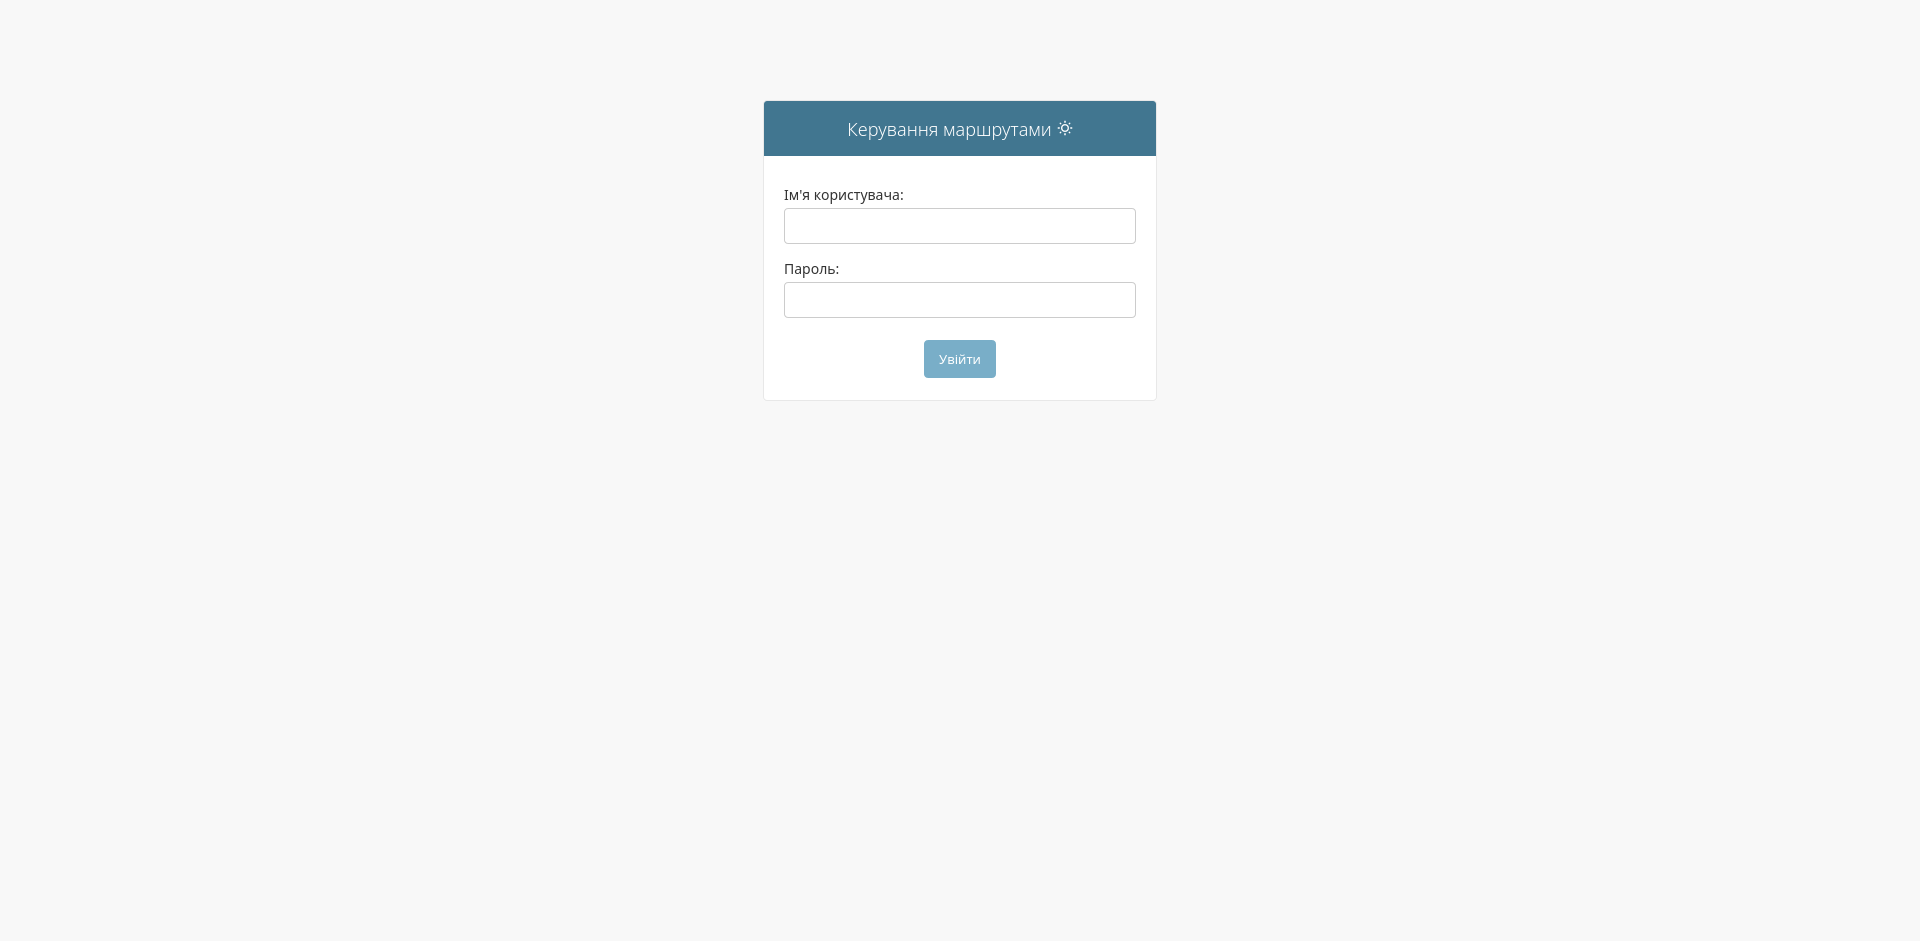
\includegraphics[scale=0.35]{content/chapters/4-results/assets/img/login_page.png}
	\caption{Сторінка входу}
	\label{fig:login_page}
\end{figure}

Можливості адміністратора буде розглянуто в наступному розділі